\section{February 14}
Last time, we showed that for waves with \( E_I \) in the incident plane, the reflected and transmitted waves
have the same polarization. That is, we found that \( \phi_R = \phi_T = 0 \). So, the six boundary conditions
we had from before now transform into:
\begin{align}
	\label{lec11:BC-1}\epsilon_1 \sin \theta_\text{in}\left( E_I - E_R \right) 
	&= \epsilon_2 \sin \theta_\text{out} E_T\\
	\label{lec11:BC-2}\cos \theta_\text{in} (E_I + E_R) &= \cos \theta_\text{out}E_T\\
	\label{lec11:BC-3}(E_I - E_R) &=  \beta E_T 
\end{align}
Reminder that \( \beta = \frac{\mu_1v_1}{\mu_2 v_2} \). Here, we see that equation \ref{lec11:BC-1} is
actually the same condition as \ref{lec11:BC-3}, but written in a different form. To see this, we have:
\[
	(E_I - E_R) = \frac{\epsilon_2 \sin \theta_\text{out}}{\epsilon_1 \sin \theta_\text{in}} E_T =
	\frac{\epsilon_2 v_2}{\epsilon_1 v_1} E_T = \frac{\mu_1v_1^2 v_2}{\mu_2v_2^2 v_1}E_T =
	\frac{\mu_1v_1}{\mu_2v_2}E_T = \beta E_T
\]
So now this means that we essentially have two boundary conditions:
\[
	E_I + E_r = \alpha E_T \quad (E_I - E_R) = \beta E_T
\]
So, we can solve for \( E_T \):
\[
	E_T = \frac{2}{\alpha + \beta} \quad E_R = \frac{\alpha - \beta}{\alpha + \beta}
\]
Now, some comments about these results. Firstly, \( E_T \) always has the same sign as \( E_I \), so this
means that the transmitted wave has no phase shift. However, depending on \( \alpha
- \beta\), the reflected wave may pick up a \( \pi \) phase shift, specifically when \( \beta > \alpha \). In
the case where we have normal incidence, then \( \alpha = 1 \), so this is why the reflected wave always
picks up a phase shift. We can also rewrite \( \alpha \):
\[
	\alpha = \frac{\cos \theta_\text{out}}{\cos \theta_\text{in}} = \frac{\sqrt{1 - \sin^2
	\theta_\text{out}}}{\cos \theta_\text{in}} = \frac{\sqrt{1 - \left( \frac{n_1}{n_2} \right)^2 \sin^2
\theta_\text{in}}}{\cos \theta_\text{in}}
\]
This results means that there is always a \( \theta_\text{in} \) such that \( \alpha - \beta = 0 \), and in
this case no reflection occurs. This \( \theta_\text{in} \) is the so-called \textbf{Brewster
angle}.\footnote{This is the reason we can attach a polarizing filter onto a camera lens and get rid of
reflections that come off the glass.}

\subsection{Brewster's Angle}
What's the explicit form of \( \theta_B	\), the critical angle? We can find \( \theta_B \) by 
setting \( \alpha = \beta \): 
\[
	\beta = \frac{\sqrt{1 - \left( \frac{n_1}{n_2} \right)^2 \sin^2 \theta_B}}{\cos \theta_B} \implies \sin^2
	\theta_B = \frac{1 - \beta^2}{\left( \frac{n_1}{n_2} \right)^2 - \beta^2 }
\]
In the case where \( \mu_2 \simeq \mu_1 \simeq \mu_0 \), then this equation becomes:
\[
	\sin^2 \theta_B = \frac{1 - \beta^2}{\frac{1}{\beta^2} - \beta^2} = \frac{\beta^2(1 - \beta^2)}{1 -
	\beta^{4}} = \frac{\beta^2}{1 + \beta^2} \implies \sin \theta_B = \frac{\beta}{\sqrt{1 + \beta^2}}
\]
We can then draw a right triangle with hypotenuse \( \sqrt{1 + \beta^2} \), which gives \( \tan \theta_B =
\frac{n_2}{n_1} \). What's the physical intuition for this phenomenon? One way you can convince yourself of
this phenomenon is to consider the microscopic picture of dipole radiation. Consider a dipole:
\begin{center}
	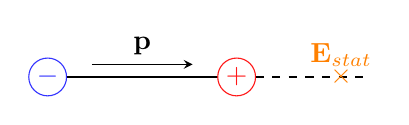
\begin{tikzpicture}[scale=0.8]
		\draw[blue!80!white] (0, 0) circle (0.3) node {\( - \)};
		\draw (0.3, 0) -- (2.7, 0);
		\draw[red!90!white] (3, 0) circle (0.3) node {\( + \)};
		\draw[dashed] (3.3, 0) -- node[pos=0.8] {\color{orange}\( \times \)} node [pos=0.8, above=0.1]
			{\color{orange} \(
			\mathbf{E}_\text{stat} \)} (5, 0); 
		\draw[-stealth] (0.7, 0.2) -- node[midway, above] {\( \mathbf{p} \)} (2.3, 0.2);
	\end{tikzpicture}
\end{center}
Now, consider the field at the point \( \mathbf{E}_\text{stat} \). The field lines can only be horizontal due
to symmetry, but this immediately means that such a field cannot be caused by a wave travelling in this
direction, since \( \mathbf{k} \perp \mathbf{E} \). Therefore, for a dipole there is no wave propagation
along the direction of the dipole moment \( \mathbf{p} \). We can also provably show this using the dipole
radiation equation, which will come in chapter 11. 

Anyways, what this means for our system is that whenever the dipoles end up oscillating in the direction that
the reflected wave would propagate in (according to the law of reflection), then there is no reflected wave.
This angle also happens to be perpendicular to \( \mathbf{k}_T \). From this observation, because \(
\mathbf{k}_T \perp \mathbf{k}_R \), then we can write: 
\[
	\theta_B + \theta_\text{out} = \frac{\pi}{2}
\]
By Snell's law, \( n_1 \sin \theta_B = n_2 \sin \theta_\text{out} = n_2 \cos \theta_B \), and indeed from
here we get the Brewster angle \( \tan \theta_B = \frac{n_2}{n_1} \). 

\subsection{Reflection and Transmission Coefficient}
Now let's go back to the diagram we made from earlier. Based on the way the waves propagate, we know that
there should be energy propagating in the \( x \) direction. By the conservation of energy, we know that \(
I_{z, \text{in}} = I_{z, \text{out}} \) along the boundary. To be specific, here \( I \) represents an
intensity, with units of energy flow per area per time. Given these units, it makes sense to use the Poynting
vector to calculate this:
\[
	|I_{z, R}| = |\mathbf{S}_R \cdot \mathbf{\hat{z}}| = \frac{E_R B_R}{\mu_1}\cos \theta_\text{in} =
	\frac{E_R^2}{\mu_1v_1} \cos \theta_\text{in}
\]
where we use the relation that \( |\mathbf{B}| = \frac{|\mathbf{E}|}{v_1} \) for waves. The incoming
intensity can also be calcualted:
\[
	|I_{z, I}| = |\mathbf{S}_I \cdot \mathbf{\hat{z}}| = \frac{E_I}{\mu_1v_1} \cos \theta_\text{in}
\]
Combining these two equations, we get:
\[
	R = \frac{|I_{z, R}|}{|I_{z, I}|} = \frac{E_R^2}{E_I^2} = \left| \frac{\alpha - \beta}{\alpha + \beta}
	\right|^2
\]
Similarly, the transmission can also be calculated as \( I_{z, T} = \frac{E_T^2}{\mu_2v_2} \cos
\theta_\text{out} \), so:
\[
	T = \frac{|I_{z, T}|}{|I_{z, I}|} = \frac{\mu_1v_1}{\mu_2v_2} \frac{|E_T|^2}{|E_I|^2}
	\frac{\cos\theta_\text{out}}{\cos\theta_\text{in}} = \alpha \beta \left( \frac{2}{\alpha + \beta}
	\right)^2
\]
Indeed, if you add these two up, you get \( R + T = 1 \), as required by conservation of energy. 

\subsection{Total Internal Reflection}

Another phenomenon that is a result of these rules is total internal reflection. This occurs when \(
\theta_\text{out} = \frac{\pi}{2} \), which gives us \( \alpha = 0 \). Looking at our formulas for \( R \)
and \( T \), this gives:
\[
	R = \left| \frac{\alpha - \beta}{\alpha + \beta} \right|^2 = 1 \quad T = \alpha \beta \left|
	\frac{2}{\alpha + \beta} \right|^2 = 0
\]
So we get no energy transmitted. What happens if we go past this critical \( \theta_c \)? Well, the effect is
that \( \sin \theta_\text{out} \) becomes imaginary. To see why, consider Snell's law:
\[
	k_I \sin \theta_I = k_T \sin \theta_T \implies \sin \theta_T = \frac{n_1}{n_2} \sin \theta_I
\]
If \( n_1 > n_2 \), then there evidently will be an angle \( \theta_I \) such that \( \sin \theta_T > 1 \),
which is not possible if we are to interpret \( \theta_T \) as an angle. One natural question one could ask
then is, instead of allowing for the possibility of \( \sin \theta_T \) to exceed 1, why not say that Snell's
law doesn't hold anymore? The reason for this is that Snell's law \textit{must} hold, as it is simply a
product of the boundary conditions imposed by Maxwell's equations. Thus, saying that Snell's law doesn't hold
is the same as saying that we violate Maxwell's equations, and of course we can't allow that. 


